\section{Experiments and Results}

\subsection{Experimental design and statistical unit}

The experiments are organized as a sequence of identification and prediction
tests rather than as an undifferentiated prompt grid. We begin with 80 latent
worlds for surface-axis discovery and a separate 80-world pressure pool for
falsification. A 30-world same-item topology matrix then crosses role, object,
and joint conflict. The same 30 worlds are rendered in four realization
families and in a construction factorial that estimates primitive voice,
locality, and source-attribution costs. We hold out 30 passive-by-embedding
forms for compound prediction and reserve 20 new latent worlds for independent
saturation confirmation. Across all matrices this produces 16,700 scored rows,
but the latent world, not the row, is the sampling unit.

The primary linguistic axes are description order, reference form, and
negation/evidential wording. Role label versus name is retained as a control and
exploratory contrast rather than promoted after inspection. Every world is
evaluated at 1,024 and 2,048 tokens with the same typed candidate interface;
neutral padding is placed outside the answer-bearing event block. This design
separates semantic invariance from surface realization and prevents context
length or candidate normalization from becoming an unreported source of
variation.

For each latent world, we average the two context lengths before resampling and
use an item-cluster bootstrap that preserves all topology, construction, and
instruction-arm rows belonging to that world. The pressure-pool reversal,
typed-topology interaction, held-out residual, and cross-checkpoint residual
therefore answer different questions. A result is promoted only when its
predeclared directional or control gate is satisfied; a failed gate remains a
boundary result rather than a reason to refit the contrast.

\subsection{Average wording effects conceal the controller}

The most economical account of prompt sensitivity is that each linguistic form
contributes a stable amount of evidence for the intended belief. Our first test
rejects that account. Description order and reference form change direction or
collapse when evaluated on an item-disjoint pressure pool. A wording form
therefore does not carry a portable, context-free weight; the complete estimates
and uncertainty intervals are reported in Appendix~\ref{tab:cross-pool}.

The first gate is a direct portability test. If a wording form carried a stable
language-level weight, its paired effect should preserve direction on the
item-disjoint pressure pool. It does not: description order reverses and
reference form collapses, while the designated controls also fail their frozen
criteria (Table~\ref{tab:main-cross-pool}). This negative result is informative
because it rules out the simplest explanation before any typed conflict probe is
introduced.

\begin{table}[H]
\centering
\footnotesize
\setlength{\tabcolsep}{3pt}
\begin{tabularx}{\columnwidth}{Xlrrrc}
\toprule
Axis & Arm & Discovery & Pressure & Sign stable & Gate \\
\midrule
Description order & Primary & -2.132 & 4.678 & No & Fail \\
Reference form & Primary & 0.705 & -0.227 & No & Fail \\
Negation/evidence & Control & 0.541 & 4.143 & Yes & Control fail \\
Role label/name & Control & -0.328 & -1.238 & Yes & Control fail \\
\bottomrule
\end{tabularx}
\caption{Cross-pool falsification of a portable wording effect. The discovery
and item-disjoint pressure pools use the same linguistic contrasts but different
latent worlds. The two preregistered primary axes reverse or collapse, so no
context-free language weight is promoted. The complete intervals and gate
definitions are reported in Appendix~D.}
\label{tab:main-cross-pool}
\end{table}


The failure points to a hidden variable: the identity of the source competing
with the target. We expose it by crossing new latent worlds with role, object,
and joint role-plus-object conflict while preserving the event sequence,
candidate vocabulary, and linguistic contrast. The joint-minus-average-single
interaction is directional for all three preregistered linguistic axes and
remains so at both context lengths (Appendix~\ref{tab:same-item}).

Table~\ref{tab:key-estimates} places the evidence on a common scale. The
typed-conflict interactions are estimated on the original worlds, whereas the
cross-realization and saturation entries are evaluated on distinct realization
families or new latent worlds. This is an evidence ladder, not a ranking of
prompt effects: each row changes the epistemic status of the claim.

\begin{table}[H]
\centering
\small
\begin{tabularx}{\columnwidth}{Xrrl}
\toprule
Estimand & Mean & Bootstrap interval & Evidence unit \\
\midrule
Order $\times$ topology & 6.722 & [5.697, 7.747] & same-world \\
Reference $\times$ topology & -1.062 & [-1.724, -0.409] & same-world \\
Negation/evidence $\times$ topology & 3.706 & [2.875, 4.527] & same-world \\
Order across realizations & 4.551 & [3.907, 5.152] & 4 realizations \\
Reference across realizations & -1.006 & [-1.474, -0.530] & 4 realizations \\
Reportative saturation & 4.609 & [2.646, 6.447] & new worlds \\
Factive saturation & 3.771 & [2.274, 5.228] & new worlds \\
\bottomrule
\end{tabularx}
\caption{Key estimates in the argument. Topology effects are joint-minus-average-single interactions; saturation effects are compound-minus-additive residuals. Intervals are 95\% percentile item-cluster bootstrap intervals.}
\label{tab:key-estimates}
\end{table}


This interaction changes the interpretation of the original instability. The
same description can help when the target competes with one source and hurt when
it competes with two. Linguistic form is not simply shifting an answer score; it
is changing arbitration among typed sources. The object to explain is therefore
\emph{source routing under conflict}, not average prompt robustness.

\subsection{A reportative reversal reveals an accessibility bottleneck}

If typed source routing is real, it should survive changes in surface
realization while remaining sensitive to constructions that alter source
access. We render the same worlds as canonical narratives, structured event
logs, event-wise reports, and compact indirect reports. Aggregate topology
effects remain directional for the main language axes, and order and reference
preserve their signs across the realization families
(Appendix~\ref{tab:multitemplate}).

The informative case is the exception. Under event-wise reportative embedding,
the negation/evidential interaction reverses direction. The event facts and
answer candidates are unchanged, but each fact now reaches the query through an
attributed report. The reversal is hard to explain as generic template
sensitivity: it specifically implicates the route from a described source to
the answer interface.

We test that interpretation by separating three ways of restricting the route:
grammatical demotion through passive voice, event-local embedding, and
reportative rather than factive attribution. Relative to the active unembedded
form, passive voice and event-local embedding each reduce the topology-moderated
effect; locality is additionally more damaging under reportative than factive
attribution. These contrasts isolate distinct linguistic restrictions on source
access without asserting that the model contains an explicit scalar
accessibility variable (Appendix~\ref{tab:factorial}).

\begin{figure*}[t]
    \centering
    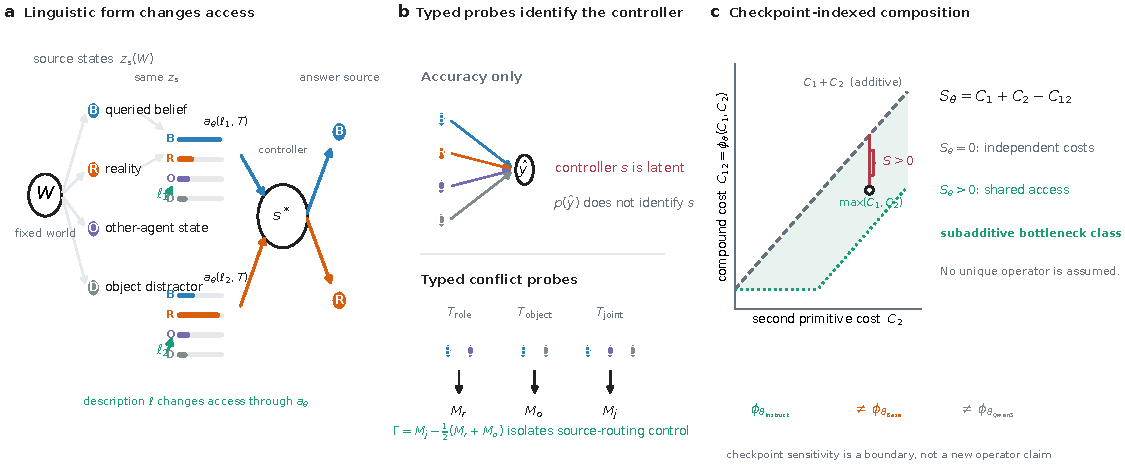
\includegraphics[width=\textwidth]{figures/figure_source_accessibility_bottleneck.pdf}
    \caption{\textbf{A theory of linguistic source control.} (a) A fixed
    latent world supplies typed source states; linguistic form changes their
    access vector and therefore the source selected at the answer interface.
    (b) Accuracy alone leaves the controller unidentifiable, whereas typed
    conflict probes produce the source-routing interaction $\Gamma$. (c) The
    compound cost lies in a subadditive class between $\max(C_1,C_2)$ and
    $C_1+C_2$. The checkpoint comparison in the final paragraph tests whether
    this composition class transfers; its complete quantitative evidence is
    reported in Table~\ref{tab:main-checkpoint-boundary}.}
    \label{fig:main}
\end{figure*}

\subsection{The bottleneck predicts subadditive composition}

The accessibility account becomes scientifically useful only if it predicts an
unseen construction. Let $c_0$ be the active, unembedded baseline, and define a
construction's behavioral accessibility cost as its loss in topology-moderated
source control relative to $c_0$. Independent restrictions predict that the
cost of passive voice and local embedding should add. A shared bottleneck
predicts overlap: once one route is limiting, the other cannot impose its full
standalone cost.

\input{../../results/oral_readiness_pack_20260707/source_accessibility_saturation_theory/source_accessibility_saturation_theorem}

Proposition~\ref{prop:cost-residual} turns this contrast into an observable
inequality. Additivity predicts $S=0$; shared saturation predicts $S>0$. The
claim is deliberately about a subadditive composition class, not a unique
weakest-link, soft-min, or neural aggregation operator.

We freeze primitive voice and locality costs before evaluating unseen
passive-by-embedding compounds. The additive model overshoots the compound
response systematically, while the saturating predictors reduce this error.
The weakest-link predictor does not reliably separate from average saturation.
The held-out compounds therefore reject independent costs and motivate a
saturating class, while leaving the operator unidentified
(Table~\ref{tab:main-heldout} and Appendix~\ref{tab:model-comparison}).

\begin{table}[H]
\centering
\footnotesize
\setlength{\tabcolsep}{3pt}
\begin{tabularx}{\columnwidth}{Xrrrrrr}
\toprule
Unseen compound & Actual & Additive & Residual & Interval & Additive MAE & No-voice MAE \\
\midrule
Passive + global reportative & -0.142 & -0.364 & 0.222 & [-0.615, 1.026] & 1.835 & 2.930 \\
Passive + local reportative & -0.757 & -3.426 & 2.668 & [2.026, 3.354] & 2.753 & 1.518 \\
Passive + global factive & 0.120 & -1.034 & 1.154 & [0.350, 1.979] & 1.967 & 2.381 \\
Passive + local factive & -0.654 & -3.066 & 2.411 & [1.707, 3.134] & 2.486 & 1.786 \\
\bottomrule
\end{tabularx}
\caption{Held-out compound test. Primitive voice and locality costs are frozen before scoring these four passive-by-embedding compounds. Three residual intervals exclude zero in the positive direction, rejecting independent additive costs. Intervals are 95\% percentile item-cluster bootstrap intervals.}
\label{tab:main-heldout}
\end{table}


\subsection{New worlds confirm the law; new checkpoints delimit it}

The decisive test freezes the residual direction and both saturating controls,
then evaluates them on latent worlds with no signature overlap with the earlier
pool. No primitive cost or operator is selected on these worlds. The compound
response lies above the additive prediction for both reportative and factive
constructions, and both saturating predictors improve over additivity. The new
worlds therefore confirm a checkpoint-internal law: concurrent linguistic
restrictions impose strictly subadditive behavioral costs in
Qwen2.5-7B-Instruct. The complete quantitative audit is provided in
Appendix~\ref{tab:independent-saturation}.

We next freeze the complete protocol and change only the checkpoint. Qwen3-8B
and matched Qwen2.5-7B Base do not reproduce the directional residual; their
intervals include zero. Yet both checkpoints retain a control-relative
preference for saturating predictors over additivity. What transfers is
therefore not the strong law itself, but a weaker structural preference
 (Table~\ref{tab:main-checkpoint-boundary}).

\begin{table}[H]
\centering
\small
\begin{tabular}{lrrcc}
\toprule
Checkpoint & Residual & Interval & Predicate gates & Control gates \\
\midrule
Qwen2.5-7B-Instruct & 4.190 & [2.931, 5.401] & 2/2 & 2/2 \\
Qwen3-8B & 0.250 & [-0.095, 0.580] & 0/2 & 2/2 \\
Qwen2.5-7B Base & -0.184 & [-0.453, 0.107] & 0/2 & 2/2 \\
\bottomrule
\end{tabular}
\caption{Frozen checkpoint boundary. The directional saturation residual is specific to Qwen2.5-7B-Instruct, whereas both alternate checkpoints retain the weaker control-relative predictor preference. Intervals are 95\% percentile item-cluster bootstrap intervals.}
\label{tab:main-checkpoint-boundary}
\end{table}


Could this be the same composition law expressed at lower confidence?
Proposition~\ref{prop:affine-gain-invariance} shows that a positive affine
readout map must preserve residual sign and normalized geometry. A
primitive-only transport fails held-out compound and residual controls for both
predicate families (Appendix~\ref{tab:affine-gain}). The cross-checkpoint
difference is therefore a change in functional composition shape, not scalar
logit compression. Strong directional saturation is associated with the
Instruct checkpoint; the evidence does not establish that instruction tuning
caused it or locate the responsible internal circuit.

Figure~\ref{fig:empirical-evidence} summarizes the empirical closure of the
argument: pooled effects reverse across item pools, the frozen additive null
overshoots held-out compounds, and the directional residual is restricted to
the Instruct checkpoint even though control-relative saturating predictors
remain useful elsewhere.

\begin{figure*}[t]
    \centering
    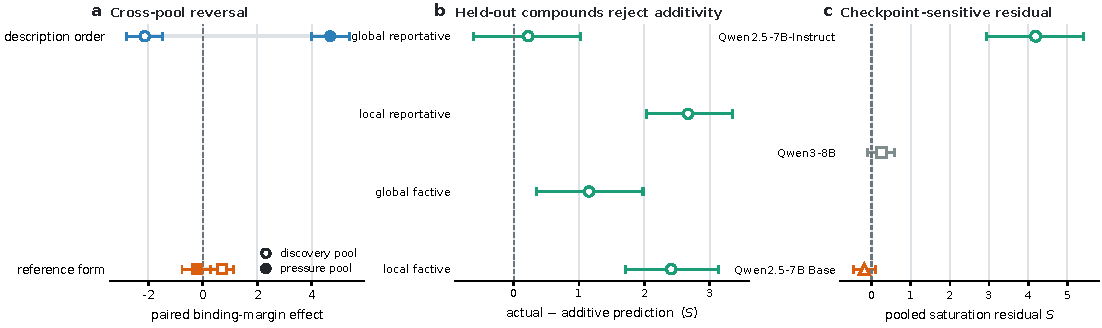
\includegraphics[width=\textwidth]{figures/figure_empirical_evidence.pdf}
    \caption{\textbf{Empirical closure of the source-accessibility argument.}
    (a) Discovery and item-disjoint pressure pools produce incompatible pooled
    wording effects. Open and filled markers denote the two pools; intervals are
    95\% item-cluster bootstrap intervals. (b) On four unseen passive-by-
    embedding compounds, actual responses exceed the frozen additive prediction
    in the positive residual direction. (c) The pooled saturation residual is
    directional only for Qwen2.5-7B-Instruct; Qwen3-8B and matched Qwen2.5-7B
    Base preserve a weaker control-relative preference but not the directional
    law.}
    \label{fig:empirical-evidence}
\end{figure*}
